\documentclass{article}
\usepackage{qilin}
\title{ESC195 Midterm Review}
\author{QiLin Xue}
\lhead{ESC195}
\rhead{QiLin Xue}

\begin{document}
    \maketitle
    \tableofcontents
    \section{L'hopital's Rule}
    When the limit of a function takes the form of $\frac{0}{0}$ or $\frac{\infty}{\infty}$, we can use L'hopital's rule:
    \begin{align}
        & \lim_{x \to a} \frac{f(x)}{g(x)} & \text{indeterminate} \\ 
        &= \lim_{x\to a} \frac{f'(x)}{g'(x)}
    \end{align}
    Not all indeterminate forms take this form however. Below is a list of indeterminate forms and how we can transform it to the one we're familiar with:
    \begin{center}
        \includegraphics[width=\linewidth]{figures/indeterminate.png}
    \end{center}
    \section{Integrals}
    A high level overview of steps that one should take when solving any integral is given in the \href{http://xueqilin.me/engsci-2t4/esc195/integral_flowchart.pdf}{flowchart}. Here are a few more tips:
    \begin{itemize}
        \item Look for symmetry. If the function is odd or even, that may come into handy!
        \item For rational functions, try adding and subtracting the same term to the numerator.
        \item You can sometimes remove rationals (i.e. square roots) with the substitution $x=u^2$.
    \end{itemize}
    \subsection{Improper Integrals}
    An improper integral is defined as:
    \begin{equation}
        \int_a^\infty f(x) \dd{x} = \lim_{b\to\infty} \int_a^b f(x) \dd{x}
    \end{equation}
    And from $-\infty$ to $\infty$, we have:
    \begin{equation}
        \int_{-\infty}^{\infty} = \int_{-\infty}^a f(x) \dd{x} + \int_a^\infty f(x) \dd{x}
    \end{equation}
    Here is an important theorem to determine when an integral converges to diverges:
    \begin{theorem}
        \textbf{Comparison Test:} Let $f,g$ be continuous functions and $0 \le f(x) \le g(x)$ where $x\in [a,\infty)$,. 
        \begin{itemize}
            \item If $\int_a^\infty g \dd{x}$ converges, so does $\int_a^\infty f(x) \dd{x}$.
            \item If $\int_a^\infty f \dd{x}$ diverges, so does $\int_a^\infty g(x) \dd{x}$.
        \end{itemize}
    \end{theorem}
    \subsection{Applications}
    Here are some things you can do with integrals:
    \begin{itemize}
        \item The arclength of a curve is:
        \begin{equation}
            s = \int_a^b \sqrt{1+f'(x)^2}\dd{x}
        \end{equation}
        \item The surface area of a surface of revolution is:
        \begin{equation}
            A =\int_a^b 2\pi f(x) \sqrt{1+f'(x)^2}\dd{x}
        \end{equation}
        \item The force a fluid exerts on the flat \textit{wall} of a container is:
        \begin{equation}
            F = \int_a^b \rho gx w(y) \dd{y}
        \end{equation} 
        where $w(y)$ is the width as a function of height $y$.
        \item The centroid of a curve is given by:
        \begin{equation}
            \bar{x} = \frac{\int_a^b xf(x) \dd{x}}{\int_a^b f(x) \dd{x}}
        \end{equation}
        and
        \begin{equation}
            \bar{y} = \frac{\int_a^b f(x)^2\dd{x}}{2\int_a^b f(x) \dd{x}}
        \end{equation}
        \item Pappus's Centroid theorem can be used to easily find the volume of revolution:
        \begin{equation}
            V = 2\pi R A
        \end{equation}
        where $R$ is the distance from the centroid to the axis of rotation and $A$ is the area of the rotated regoin.
        \item Similarly, we can also extend this to the centroid, which tells us that the surface area of a surface of revolution is:
        \begin{equation}
            A = 2\pi R d
        \end{equation}
        where $d$ is the arclength of the curve.
    \end{itemize}
    \section{Parametric Equations}
    Parametric equations are parametized by $x(t)$ and $y(t)$. As a result, they form a plane curve.
    \begin{itemize}
        \item The derivative of the function at time $t$ is given by:
        \begin{equation}
            \frac{dy}{dx} = \frac{y'(t)}{x'(t)}
        \end{equation}
        \item The area of a parametric curve is given by:
        \begin{equation}
            A = \int_{t_1}^{t_2} y(t)x'(t) \dd{t}
        \end{equation}
        \item For a closed loop, the area can be represented in two ways:
        \begin{equation}
            A = -\int_{t_1}^{t_2} y(t)x'(t) \dd{t} = \int_{t_1}^{t_2} x(t)y'(t) \dd{t}
        \end{equation}
        where $t_1$ and $t_2$ correspond to the same location. By convention, the curve has positive area when traversed counterclockwise.
        \item The arclength can be written as:
        \begin{equation}
            s = \int_\alpha^\beta \sqrt{1+f'(x)^2}\dd{x}
        \end{equation}
        \item The surface area when the curve is revolved is given by:
        \begin{equation}
            A = \int_{t_1}^{t_2} 2\pi y(t)\sqrt{x'(t)^2+y'(t)^2} \dd{t}
        \end{equation}
    \end{itemize}
    \subsection{Graphing}
    If possible (and if it is easy), convert the parametric equations to a cartesian equation and plot it normally. If the above will make the problem significantly harder, here is a checklist to plot a parametric function:
    \begin{itemize}
        \item Check for potential vertical tangents by setting $x'(t)=0$.
        \item Check for potential horizontal tangents by setting $y'(t)=0$.
        \item Find $x$ and $y$ intercepts by setting $x(t)=0$ and $y(t)=0$.
        \item Look for periodicity in either $x$, $y$, or both.
        \item Find the coordinate and the slope $\frac{dy}{dx}$ at $t=0$ and at the endpoint $t=t_f$.
        \item Is $x(t)$ a $1-1$ function? If not, you'll get a graph where some points are directly above others.
    \end{itemize}
    \subsection{Common Parametric Curves}
    Here is a list of common parametric curves:
    \begin{itemize}
        \item A circle centered at $(x_0,y_0)$ with radius $r$:
        \begin{equation}
            (x_0 + r\cos(\pm \omega t), y_0 + r\sin(\pm \omega t))
        \end{equation}
        where $\omega \in \mathbb{R}$.
        \item An ellipse centered at $(x_0,y_0)$ with a horizontal length $a$ and vertical length $b$:
        \begin{equation}
            (x_0 + a\cos(\pm \omega t), y_0+ b\sin(\pm \omega t))
        \end{equation}
        where $\omega \in \mathbb{R}$.
        \item A straight line with slope $m$ passing through $(x_0,y_0)$:
        \begin{equation}
            (x_0 + at, y_0 + amt)
        \end{equation}
        where $a \in \mathbb{R}$.
        \item A \textbf{cycloid} (e.g. the curve traced by a point on a rolling circle with radius $a$ with angular frequency $\omega$) is given by:
        \begin{equation}
            (a\omega t-a\sin \omega t, a-a\cos\omega t)
        \end{equation}
        which is seen in the below diagram:
        \begin{center}
            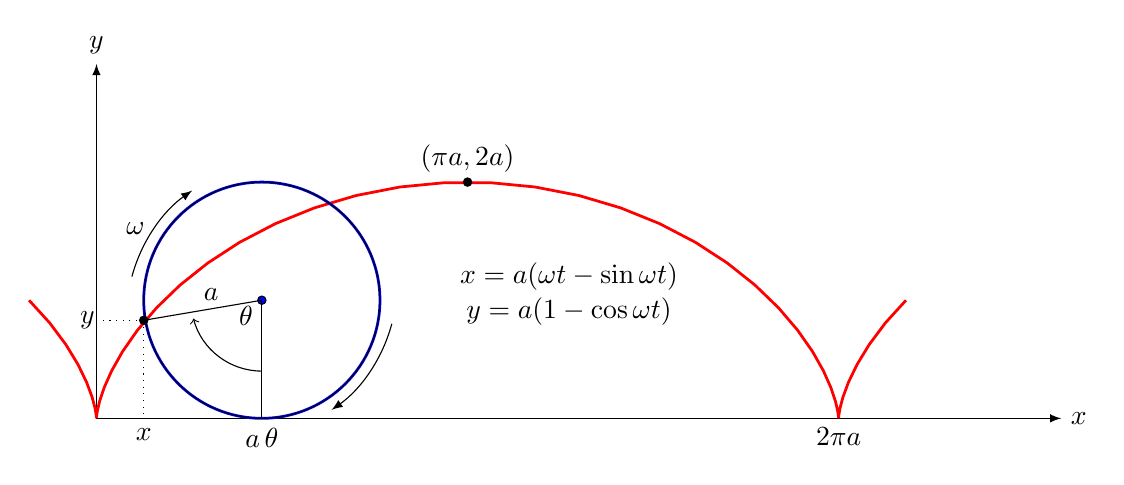
\begin{tikzpicture}[scale=1.5]
            \coordinate (O) at (0,0);
            \coordinate (A) at (0,3);
            \def\r{1} % radius
            \def\c{1.4} % center
            \coordinate (C) at (\c, \r);
          
          
            \draw[-latex] (O) -- (A) node[anchor=south] {$y$};
            \draw[-latex] (O) -- (2.6*pi,0) node[anchor=west] {$x$};
            \draw[red,domain=-0.5*pi:2.5*pi,samples=50, line width=1] 
                 plot ({\x - sin(\x r)},{1 - cos(\x r)});
            \draw[blue, line width=1] (C) circle (\r);
            \draw[] (C) circle (\r);
          
            % coordinate x 
            \def\x{0.4} % coordinate x
            \def\y{0.83} % coordinate y
            \def\xa{0.3} % coordinate x for arc left
            \def\ya{1.2} % coordinate y for arc left
            \coordinate (X) at (\x, 0 );
            \coordinate (Y) at (0, \y );
            \coordinate (XY) at (\x, \y );
          
            \node[anchor=north] at (X) {$x$} ;
          
            % draw center of circle
            \draw[fill=blue] (C) circle (1pt);
          
            % draw radius of the circle
            \draw[] (C) -- node[anchor=south] {\; $a$} (XY);
          
            % bottom of circle, radius to the bottom
            \coordinate (B) at (\c, 0);
            \draw[] (C) -- (B) node[anchor=north] {$a \, \theta$};
          
            % projections of point XY
            \draw[dotted] (XY) -- (X);
            \draw[dotted] (XY) -- (Y) node[anchor=east, xshift=1mm] {$\quad y$};
          
            % arc theta
            % start arc
            \coordinate (S) at (\c, 0.4);
            \draw[->] (S) arc (-90:-165:0.6);
            \node[xshift=-2mm, yshift=-2mm] at (C) { $\theta$};
          
            % arc above
            \coordinate (AA) at (\xa, \ya);
            \draw[-latex, rotate=25] (AA) arc (-220:-260:1.3)node[midway,left] {$\omega$} ;
          
            % arc below
            \def\xb{2.5} % coordinate x for arc bottom
            \def\yb{0.8} % coordinate y for arc bottom
            \coordinate (AB) at (\xb, \yb);
            \draw[-latex, rotate=-10] (AB) arc (-5:-45:1.3);
          
          
          
            % XY dot
            \draw[fill=black] (XY) circle (1pt);
          
          
            % top label
            \coordinate (T) at (pi, 2);
            \node[anchor=south] at (T)  {$(\pi a, 2 a )$} ;
            \draw[fill=black] (T) circle (1pt);
          
            % equations
            \coordinate (E) at ( 4,1.2);
            \coordinate (F) at ( 4,0.9);
            \node[] at (E) { $x=a(\omega t - \sin \omega t)$};
            \node[] at (F) { $y=a(1 - \cos \omega t)$};
          
            % label 2pi a
            \coordinate (TPA) at (2*pi, 0);
            \node[anchor=north] at (TPA) {$2 \pi a$};
          
          
            \end{tikzpicture}
          \end{center}
          \item An \textbf{astroid} is given by:
          \begin{equation}
              (a\cos^3 \omega t, a\sin^3 \omega t)
          \end{equation}
          which represents the curve traced out by a point on a rolling circle with radius $a/4$ rolling inside a circle of radius $a$.
          \begin{center}            \begin{tikzpicture}
            \begin{axis}[
            trig format plots=rad,
            legend pos=outer north east,
            title=Astroid,
            axis lines = box,
            axis equal image,
            xlabel = $x$,
            ylabel = $y$,
            ]
            \addplot [domain=0:2*pi, samples=100, red] ({cos(x)^3}, {sin(x)^3});
            \end{axis}
            \end{tikzpicture}
        \end{center}
        % \item A hypocycloid describes a general class of curves of the above type (i.e. circle rolling inside other circle of radius $a$). If it has $n$ cusps, then:
        % \begin{equation}
        %     \left(\frac{n-1}{n}(a\cos t) + \frac{a}{n}\cos((n-1)\omega t), \frac{n-1}{n}(a\sin t) + \frac{a}{n}\sin((n-1)\omega t)\right)
        % \end{equation}
        % Too complicated
    \end{itemize}
    \section{Polar Curves}
    Polar curves are another type of plane curve defined using polar coordinates $[r, \theta]$. We can convert between cartesian and polar coordinates using the following transformations:
    \begin{align}
        x &= r\cos\theta \\ 
        y &= r\sin\theta \\ 
        r &= \sqrt{x^2+y^2} \\ 
        \theta &= \arctan\left(\frac{y}{x}\right)
    \end{align}
    Calculus related results are summarized below:
    \begin{itemize}
        \item The derivative is given by:
        \begin{equation}
            \frac{dy}{dx} = \frac{\frac{dr}{d\theta}\sin\theta + r\cos\theta}{\frac{dr}{d\theta}\cos\theta - r\sin\theta}
        \end{equation}
        \item The area is given by:
        \begin{equation}
            A = \frac{1}{2}\int_\alpha^\beta r(\theta)^2 \dd{\theta}
        \end{equation}
        \item The arclength is given by:
        \begin{equation}
            s = \int_\alpha^\beta \sqrt{r^2+\left(\frac{dr}{d\theta}\right)^2} \dd{\theta}
        \end{equation}
    \end{itemize}
    \subsection{Graphing}
    Here is a checklist for plotting polar graphs:
    \begin{itemize}
        \item Check for symmetry:
        \begin{itemize}
            \item Symmetry about $x$ axis: $r(\theta)=r(-\theta)$
            \item Symmetry about $y$ axis: $r(\pi-\theta) = r(\theta)$
            \item Symmetry about origin: $r(\theta) = r(\theta+\pi)$
        \end{itemize}
        \item Check the domain
        \item Find when $r=0$
        \item Find local max and min values of $r$ and where they are located, and break it up into intervals.
        \item It isn't always necessary but it may help to calculate $\frac{dy}{dx}$ at important locations.
    \end{itemize}
    \subsection{Common Polar Curves}
    Note that the orientation of the below curves are not always fixed. It is possible to flip and rotate them by shifting the argument $\theta$ or using negative numbers. They just represent the general class of functions.
    \begin{itemize}
        \item Straight lines:
        \begin{itemize}
            \item Straight lines $y=mx$: can be represented by $\theta = \arctan(m)$.
            \item Vertical lines $x=a$: can be represented by $r=a\sec\theta$.
            \item Horizontal lines $y=b$: can be represented by $r=b\csc\theta$.
        \end{itemize}
            \item Circles:
            \begin{equation}
                r = -2\cos\theta
            \end{equation}
            \begin{center}
                \begin{tikzpicture}
                    \draw[thick,->,>=latex] (-3,0)--(3,0) node[above] {$x$};
                    \draw[thick,->,>=latex] (0,-3)--(0,3) node[left] {$y$};
                    \draw[domain=0:540,scale=1.5,samples=500] plot (\x:{-2*cos(\x)});
                \end{tikzpicture}
            \end{center}
            \item \textbf{Cardioids}:
            \begin{equation}
                r= a + a\cos\theta 
            \end{equation}
    
            \begin{center}
                \begin{tikzpicture}
                    \draw[thick,->,>=latex] (-3,0)--(3,0) node[above] {$x$};
                    \draw[thick,->,>=latex] (0,-3)--(0,3) node[left] {$y$};
                    \draw[domain=0:540,scale=1.5,samples=500] plot (\x:{1+1*cos(\x)});
                \end{tikzpicture}
            \end{center}
            \item \textbf{Limacons}:
            \begin{equation}
                r=a+b\sin\theta
            \end{equation}
            There are two types, for $a>b$:
            \begin{center}
                \begin{tikzpicture}
                    \draw[thick,->,>=latex] (-3,0)--(3,0) node[above] {$x$};
                    \draw[thick,->,>=latex] (0,-3)--(0,3) node[left] {$y$};
                    \draw[domain=0:540,scale=1.5,samples=500] plot (\x:{1+0.5*cos(\x)});
                \end{tikzpicture}
            \end{center}
            For $a<b$:
            \begin{center}
                \begin{tikzpicture}
                    \draw[thick,->,>=latex] (-3,0)--(3,0) node[above] {$x$};
                    \draw[thick,->,>=latex] (0,-3)--(0,3) node[left] {$y$};
                    \draw[domain=0:540,scale=1.5,samples=500] plot (\x:{0.5+1*cos(\x)});
                \end{tikzpicture}
            \end{center}
            \item \textbf{Leminiscates}. Again, there are two types. For:
            \begin{equation}
                r^2 = a\sin(2\theta)
            \end{equation}
            \begin{center}
                \begin{tikzpicture}
                    \draw[thick,->,>=latex] (-3,0)--(3,0) node[above] {$x$};
                    \draw[thick,->,>=latex] (0,-3)--(0,3) node[left] {$y$};
                    \draw[domain=0:90,scale=1.5,samples=500] plot (\x:{sqrt(sin(2*\x))});
                    \draw[domain=0:90,scale=1.5,samples=500] plot (\x:{-sqrt(sin(2*\x))});
                \end{tikzpicture}
            \end{center}
            and:
            \begin{equation}
                r^2 = a\cos(2\theta)
            \end{equation}
            \begin{center}
                \begin{tikzpicture}
                    \draw[thick,->,>=latex] (-3,0)--(3,0) node[above] {$x$};
                    \draw[thick,->,>=latex] (0,-3)--(0,3) node[left] {$y$};
                    \draw[domain=-45:45,scale=1.5,samples=500] plot (\x:{sqrt(cos(2*\x))});
                    \draw[domain=-45:45,scale=1.5,samples=500] plot (\x:{-sqrt(cos(2*\x))});
                \end{tikzpicture}
            \end{center}
            \item \textbf{Petal curves}:
            \begin{align}
                r &= a\sin(n\theta) \\ 
                r &= a\cos(n\theta)
            \end{align}
            where $n$ is an integer. There are $n$ petals if $n$ is odd and $2n$ petals if $n$ is even. For example, the following is: $r=2\cos 3\theta$:
            \begin{center}
                \begin{tikzpicture}
                    \draw[thick,->,>=latex] (-3,0)--(3,0) node[above] {$x$};
                    \draw[thick,->,>=latex] (0,-3)--(0,3) node[left] {$y$};
                    \draw[domain=0:360,scale=1.5,samples=500] plot (\x:{2*cos(3*\x)});
                \end{tikzpicture}
            \end{center}
            and for $r=2\sin(4\theta)$:
            \begin{center}
                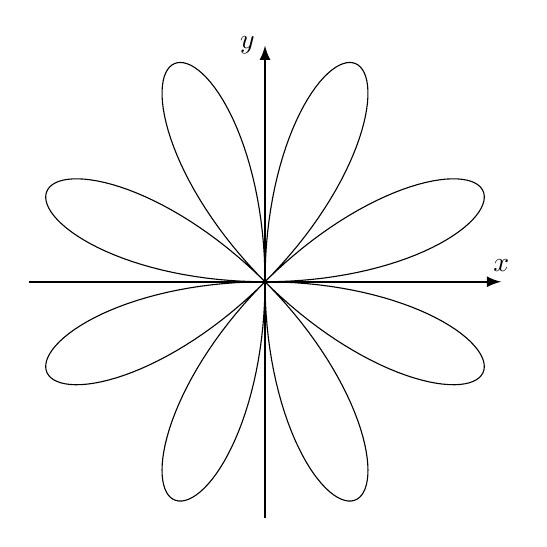
\begin{tikzpicture}
                    \draw[thick,->,>=latex] (-3,0)--(3,0) node[above] {$x$};
                    \draw[thick,->,>=latex] (0,-3)--(0,3) node[left] {$y$};
                    \draw[domain=0:360,scale=1.5,samples=500] plot (\x:{2*sin(4*\x)});
                \end{tikzpicture}
            \end{center}
    \end{itemize}
\end{document}